\documentclass[a4paper,12pt]{extarticle} %размер бумаги устанавливаем А4, шрифт 12пунктов
\usepackage[T2A]{fontenc}
\usepackage[utf8]{inputenc}%включаем свою кодировку: koi8-r или utf8 в UNIX, cp1251 в 

\usepackage[english,russian]{babel}%используем русский и английский языки с переносами
\usepackage{amssymb,amsfonts,amsmath,mathtext,cite,enumerate,float,bm} %подключаем 
\usepackage[colorlinks=True,urlcolor=blue]{hyperref}
%\usepackage{caption2} %Чтобы поменять двоеточие в названии таблицы на тире
%\renewcommand{\rmdefault}{ftm}

\usepackage{geometry}
\geometry{left=3cm}
\geometry{right=1.5cm}
\geometry{top=2.4cm}
\geometry{bottom=2.4cm}

\renewcommand{\baselinestretch}{1.5}  % 1 интервал

\renewcommand{\thetable}{\arabic{section}.\arabic{table}}

%\renewcommand{\captionlabeldelim}{ \textendash}

\tolerance=10000

\newcommand{\D}{\mathrm{d}}
% Производные
\newcommand{\dsl}[2]{{\partial #1}/{\partial #2}}
\newcommand{\df}[1]{\cfrac{\partial}{\partial #1}}
\newcommand{\dff}[2]{\frac{\partial #1}{\partial #2}}
\newcommand{\dfs}[2]{\frac{\partial^2 #1}{\partial #2^2}}
\newcommand{\Df}[1]{\frac{d}{d #1}}
\newcommand{\Dff}[2]{\frac{d #1}{d #2}}
\newcommand{\Dfs}[2]{\frac{d^2 #1}{d #2^2}}
\newcommand{\cDf}[1]{\cfrac{d}{d #1}}
\newcommand{\cDff}[2]{\cfrac{d #1}{d #2}}
\newcommand{\cDfs}[2]{\cfrac{d^2 #1}{d #2^2}}
\newcommand{\dfn}[3]{\frac{\partial^#1 #2}{\partial^#1 #3}}
% Векторы
\renewcommand{\vec}[1]{\bm{#1}}
\newcommand{\ort}[1]{\bm{\mathrm{e}}_#1}
% Векторный анализ
\renewcommand{\div}{\mathrm{div}\,}
\newcommand{\rot}{\mathrm{rot}\,}
\newcommand{\grad}{\mathrm{grad}\,}
\newcommand{\laplas}[4]{\dfs{#1}{#2}+\dfs{#1}{#3}+\dfs{#1}{#4}}
\newcommand{\laplasxyz}[1]{\dfs{#1}{x}+\dfs{#1}{y}+\dfs{#1}{z}}
\newcommand{\rotc}[4]{\dff{#1}{#2} - \dff{#3}{#4}}
\newcommand{\rotcx}[3]{\dff{#1\vphantom{E}_#3}{#2} - \dff{#1\vphantom{E}_#2}{#3}}
% Функции
\renewcommand{\cosh}{\mathrm{ch}\,}
\renewcommand{\sinh}{\mathrm{sh}\,}
\renewcommand{\tanh}{\mathrm{th}\,}
\renewcommand{\Im}{\mathrm{Im}\,}
\renewcommand{\Re}{\mathrm{Re}\,}
\renewcommand{\det}[4]{#1 #4 - #2 #3}
\renewcommand{\matrix}[4]{\begin{pmatrix}#1 & #2 \\ #3 & #4\end{pmatrix}}
\newcommand{\matrixw}[5]{\begin{#5matrix}#1 & #2 \\ #3 & #4\end{#5matrix}} % #5 = b p s v V
\newcommand{\col}[2]{\begin{pmatrix}#1 & #2\end{pmatrix}}
\newcommand{\colw}[3]{\begin{#3matrix}#1 & #2 \end{#3matrix}} % #3 = b p s v V
\newcommand{\row}[2]{\begin{pmatrix}#1 \\ #2\end{pmatrix}}
\newcommand{\roww}[3]{\begin{#3matrix}#1 \\ #2 \end{#3matrix}} % #3 = b p s v V
\newcommand{\matrixrot}[2]{\begin{#2matrix} \ort{x} & \ort{y} & \ort{z} \\ \df{x} & \df{y} & \df{z} \\ #1_x & #1_y & #1_z \end{#2matrix}}
\newcommand{\matrixrotr}[4]{\begin{#4matrix} \ort{x} & \ort{y} & \ort{z} \\ \df{x} & \df{y} & \df{z} \\ #1 & #2 & #3 \end{#4matrix}}
\newcommand{\eps}{\varepsilon}
\renewcommand{\phi}{\varphi}

\newcommand{\shtr}{\mathop{\!\vphantom{E}'}}
\newcommand{\ind}[1]{\mathop{\!\vphantom{E}_{#1}}}
%\renewcommand{\theequation}{\arabic{section}.\arabic{equation}}

\usepackage[pdftex]{graphicx}

\begin{document}

\section{Поля гребенчатой замедляющей структуры}

Рассмотрим структуру представленную на рисунке \ref{ris1}.

\begin{figure}[ht]\label{ris1}
	\centering
	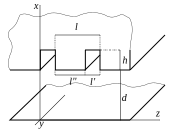
\includegraphics[width=.5\textwidth]{images/pdf/comb-type_structure.pdf}
	\caption{Гребенчатая замедляющая структура}
\end{figure}

Уравнения Максвелла в отсутствии зарядов внутри системы:
\begin{align*}
	& \div \vec{E} = 0, \\
	& \div \vec{B} = 0, \\
	& \rot \vec{E} = - \dff{\vec{B}}{t}, \\
	& \rot \vec{B} = \frac{1}{c^2}\dff{\vec{E}}{t}.
\end{align*}

Граничные условия для системы имеют вид:
\begin{align*}
	E_\text{кас}\Big|_{\text{на поверхности структуры}} = 0.
\end{align*}

Разбиваем систему на две области. Первая область -- пространство взаимодействия $0<z<d$ (далее $e$), вторая область -- область резонаторов $d<z<d+h$ (далее $r$). Ищем только поля, меняющиеся по гармоническому закону:
\begin{align*}
	& \vec{E}^{(r)} = \vec{E}^{(r)}(x, z) e^{i \omega t} \\
	& \vec{B}^{(r)} = \vec{B}^{(r)}(x, z) e^{i \omega t} \\
	& \vec{E}^{(e)} = \vec{E}^{(e)}(x, z) e^{i \omega t} \\
	& \vec{B}^{(e)} = \vec{B}^{(e)}(x, z) e^{i \omega t}
\end{align*}

Так как система однородна в направлении оси $y$, зависимости от $y$ нет. В силу периодичности системы решение в пространстве взаимодействия нужно искать в форме ряда Фурье:
\begin{align*}
& \vec{E}^{(e)}(x, z) = \sum_{n = -\infty}^{\infty} \vec{E}^{(e)}_n(x) e^{2\pi n z i /l} \\
& \vec{B}^{(e)}(x, z) = \sum_{n = -\infty}^{\infty} \vec{B}^{(e)}_n(x) e^{2\pi n z i /l}
\end{align*}

Далее $\beta_n = 2 \pi n/l$. Подставляем решения в таком виде в уравнения Максвелла и интегрируем от 0 до $l$ по $z$. Получаем:
\begin{align}
& \Dff{E^{(e)}_{nx}}{x} + i \beta_n E^{(e)}_{nz} = 0 									\label{eqp1}\\
& \Dff{B^{(e)}_{nx}}{x} + i \beta_n B^{(e)}_{nz} = 0 									\label{eqp2}\\ 
& - i \beta_n E^{(e)}_{ny} = - i \omega B^{(e)}_{nx} 									\label{eqp3}\\
& i \beta_n E^{(e)}_{nx} - \Dff{E^{(e)}_{nz}}{x} = - i \omega B^{(e)}_{ny} 				\label{eqp4}\\
& \Dff{E^{(e)}_{ny}}{x} = - i \omega B^{(e)}_{nz} 										\label{eqp5}\\
& - i \beta_n B^{(e)}_{ny} = i \frac{1}{c^2} \omega E^{(e)}_{nx} 						\label{eqp6}\\
& i \beta_n B^{(e)}_{nx} - \Dff{B^{(e)}_{nz}}{x} = i \frac{1}{c^2} \omega E^{(e)}_{ny} 	\label{eqp7}\\
& \Dff{B^{(e)}_{ny}}{x} = i \frac{1}{c^2} \omega E^{(e)}_{nz}							\label{eqp8}
\end{align}

(\ref{eqp5}) и (\ref{eqp8}) вместе с (\ref{eqp3}) и (\ref{eqp6}) эквивалентны (\ref{eqp1}) и (\ref{eqp2}). Остальные уравнения приводят к системе:
\begin{align*}
& \Dfs{B^{(e)}_{nx}}{x} - \left(\beta_n^2 - \frac{\omega^2}{c^2}\right) B^{(e)}_{nx}  =  0 \\
& \Dfs{E^{(e)}_{nx}}{x} - \left(\beta_n^2 - \frac{\omega^2}{c^2}\right) E^{(e)}_{nx}  =  0
\end{align*} 


\end{document}
